\section{Evaluation}

\subsection{Trend analysis evaluation}
To evaluate our result, we first try to show that our trend analysis
works well. To do that, we collect other document with topic label.
With these test set, its trend analysis result indirectly shows our
accuracy of trend analysis.
\subsection{Selecing test set}
We use reuters data set. It consists of more than 9000 documents
with more than 70 topics. But, the similairty of document is important
because evaluation on very diffrent set of doucments dosen't imply
any meaningful result. To resolve that, we decided to extract 10 topics
with most similairty between our dataset. It is achived by calculating
document similarity between reuters dataset and our news dataset.

To pick most similar topic, we compute maximum similairty within documents
in topic and minimum similairty bewteen reuters and news dataset. Due to
largeness of dataset, we choose only subset of dataset to calculate
minimum/maximum similairty bewteen groups.

\subsection{Reuters evaluation}
With reuters dataset with 10 pre-classified topics, we generate LDA
model for reuters dataset and make 10 topics. And we classified the topic
with given label. In result, we successfuly classified 7 topics from
LDA result. It shows that our LDA model seems to work correctly.

\begin{figure}[!htbp]
  \centering
  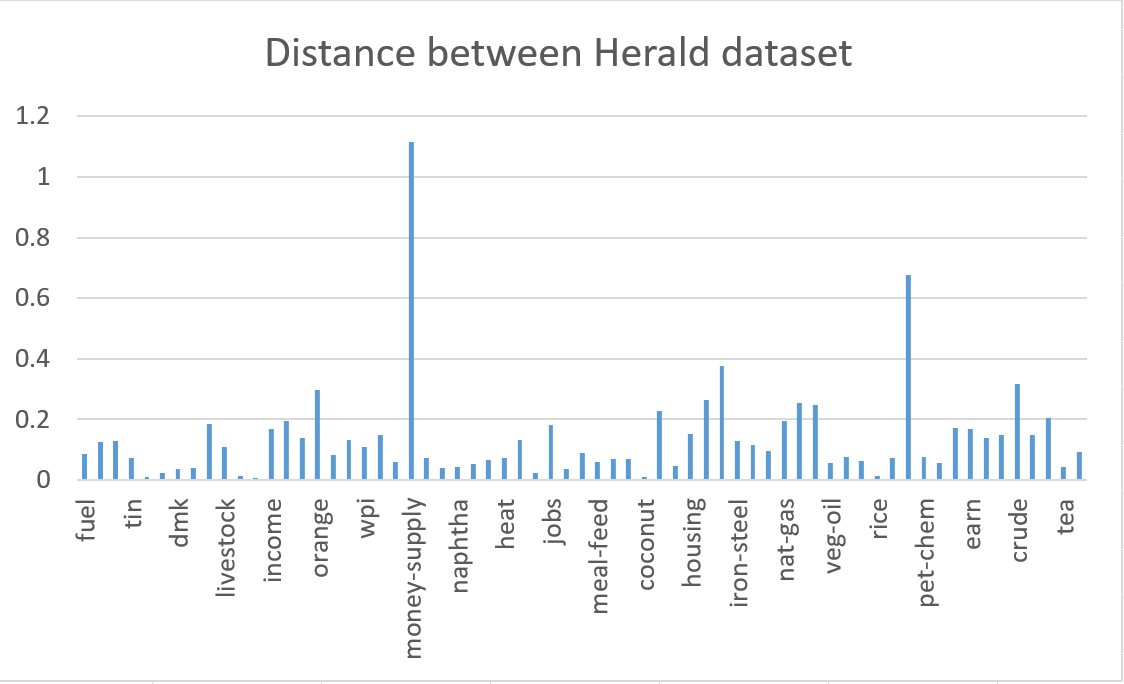
\includegraphics[width=0.8\linewidth]{Distance1}
  \caption{A brief diagram of on-issue tracking process.}
  \label{fig:onissuedia}
\end{figure}

\begin{table}[!htbp]
  \begin{tabular}{l|l}
  Topic & distance \\ \hline
  yen & 0.0061 \\
  lumber & 0.0524 \\
  veg-oil & 0.0566 \\
  strategic-metal & 0.0576 \\
  carcass & 0.0593 \\
  metal-feed & 0.0606 \\
  gold & 0.0622 \\
  ship & 0.0681 \\
  cocoa & 0.0718 \\
  oilseed & 0.0731
  \end{tabular}
  \caption{The example of on-issue tracking of the issue MERS.}
  \label{table:onissue}
\end{table}


\begin{table}[!htbp]
  \begin{tabular}{l|l}
  Group & distance \\ \hline
  nearest 10 topics & 0.061 \\
  other topics & 0.1964
  \end{tabular}
  \caption{The example of on-issue tracking of the issue MERS.}
  \label{table:onissue}
\end{table}



\subsection{Off-issue tracking}

\begin{table}[!htbp]
  \begin{tabular}{l|l|l|l|l}
  Epsilon   & $\max \Delta_{k}$ & $\min \delta(C_{i}, C_{j})$ & $DI_{m}$ & \# of cluster \\ \hline
  3 &  8.122 & 192.0 & 24.26 & 5 \\
  5 &  22.23 & 163.2 & 7.34 & 12 \\
  7 &  52.72 & 138.4 & 2.625 & 16  \\
  9 & 106.7 & 102.1 & 0.9564 & 28
  \end{tabular}
  \caption{The example of on-issue tracking of the issue MERS.}
  \label{table:onissue}
\end{table}
